To obtain a measure of success in the attempts of solving the MDP two simple baselines were implemented. The first was an idle policy, which would always return zero actions. The cumulative reward for this policy is exemplary shown for the first episode in \ref{fig:reward_idle}. The second baseline was the following threshold policy:
\begin{equation}
    a_t = \left\{
        \begin{array}{ll}
            \begin{bmatrix} \phantom{-}1 & 1 & \psi0.1 \end{bmatrix} & \text{if } I_t < \phi_1 \\
            \begin{bmatrix} -1 & 0 & \phantom{\psi}0\phantom{.1} \end{bmatrix} & \text{if } I_t > \phi_2 \\
            \begin{bmatrix} \phantom{-}0 & 0 & \psi0.1 \end{bmatrix} & \text{else}
        \end{array}
    \right.
\end{equation}
where $\phi_1$ and $\phi_2$ are the lower and upper threshold respectively, while $\psi = sign(T_t -\frac{T_{max} + T_{min}}{2})$.
\begin{figure}[H]
    \centering
    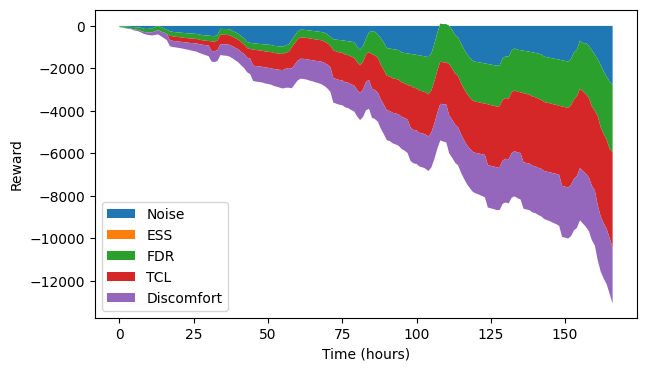
\includegraphics[width=0.45\textwidth]{figures/idle_reward.png}
    \caption{Cumulative reward for the idle policy.}
    \label{fig:reward_idle}
\end{figure}

As learning agents, Soft Actor Critic (SAC) \cite{Haarnoja.04.01.2018} and Proximal Policy Optimization (PPO) \cite{Schulman.20.07.2017} were chosen. Both implementations were taken from stable baselines 3 \cite{AntoninRaffin.2021}, and therefore only their core idea is explained.
\par
SAC is a squashed Gaussian policy, that employs entropy regularization, which adds a bonus reward in each timestep proportional to the current entropy of the policy in an aim to encourage exploration. Furthermore, two Q-functions are learned and their minimal estimate is used to update the policy. The objective function for SAC is:
\begin{equation}
    \max _\theta \underset{\substack{s \sim \mathcal{D} \\ \xi \sim \mathcal{N}}}{\mathbb{E}}\left[\min _{j=1,2} Q_{\phi_{\hat{j}}}\left(s, \tilde{a}_\theta(s, \xi)\right)-\alpha H(\pi_\theta \mid s)\right]
\end{equation}
where $\theta$ denotes the policy parameter, $\xi$ normal Gaussian noise, $\tilde{a}_\theta(s, \xi)$ the action sampled from the current policy, $\alpha$ the entropy regularization coefficient, and $H(\pi_\theta \mid s) = \log \pi_\theta\left(\tilde{a}_\theta(s, \xi) \mid s\right)$ the entropy of the policy. The action samples are obtained as $\tilde{a}_\theta(s, \xi) = tanh(\mu_\theta(s)+\sigma_\theta(s) \odot \xi)$
\par
PPO is a trust-region based policy gradient method, which solves a constrained policy update policy via SGD. It achieves the trust region remarably simple, by employing the following update objective:
\begin{flalign}
    \theta_{k+1} &= \arg \max _{\theta} \underset{\substack{s \sim \mathcal{D} \\ a \sim \pi_{\theta_k}}}{\mathbb{E}} \left[ L(s,a)\right]&& \\
    L(s,a)&=\min \left(\left|\frac{\pi_\theta(a \mid s)}{\pi_{\theta_k}(a \mid s)}\right|, 1\pm \epsilon \right) A^{\pi_{\theta_k}}(s, a)&&
    \normalsize
\end{flalign}
where $A^{\pi_{\theta_k}}(s, a)$ is the advantage of the current policy, and $\epsilon$ the trust region hyperparameter, clipping the update size. Alternatively, PPO can also be implemented using a KL-divergence constraint.